\subsection{Ukulele Tabs}

Ukulele Tabs es una aplicación web dedicada exclusivamente al ukelele. Entre las páginas que componen la aplicación distinguimos las relacionadas con canciones, herramientas y las informativas.

En primer lugar, con respecto a las \textbf{páginas relacionadas con canciones}, podemos encontrar:

\begin{itemize}
    \item \textbf{Biblioteca de canciones} (véase Figura~\ref{fig:ukuleletabs_home}), con la posibilidad de realizar búsquedas avanzadas por género, artista, popularidad, dificultad, año o país.
    \item \textbf{Canciones} (véase Figura~\ref{fig:ukuleletabs_somewhereovertherainbow}) que contienen la letra, acordes y utilidades (véase Tabla~\ref{tab:ukuleletabs_utilidades_canciones}) para la práctica de las mismas.
    

    \item \textbf{Solicitudes} de nuevas canciones.
\end{itemize}

En segundo lugar, en cuanto a las \textbf{páginas de herramientas e informativas}, distinguimos:

\begin{itemize}
    \item \textbf{Cursos} (véase Figura~\ref{fig:ukuleletabs_lecciones}), con publicaciones destinadas a la enseñanza del instrumento, principios básicos musicales y técnicas intermedias y avanzadas.
    \item \textbf{Diccionario de acordes}, con un listado de tablas con diagramas de acordes.
    \item \textbf{Calculadora de escalas y notas} (véase Figura~\ref{fig:ukuleletabs_escalas}), que muestra la ubicación de las notas en una simulación del mástil del instrumento.
    \item  \textbf{Bibliotecas de sonido} para escuchar rasgueos y afinar el instrumento a oído.
\end{itemize}

\begin{figure}[H]
    \centering
    % Primera subfigura
    \begin{subfigure}[t]{0.48\textwidth}
        \centering
        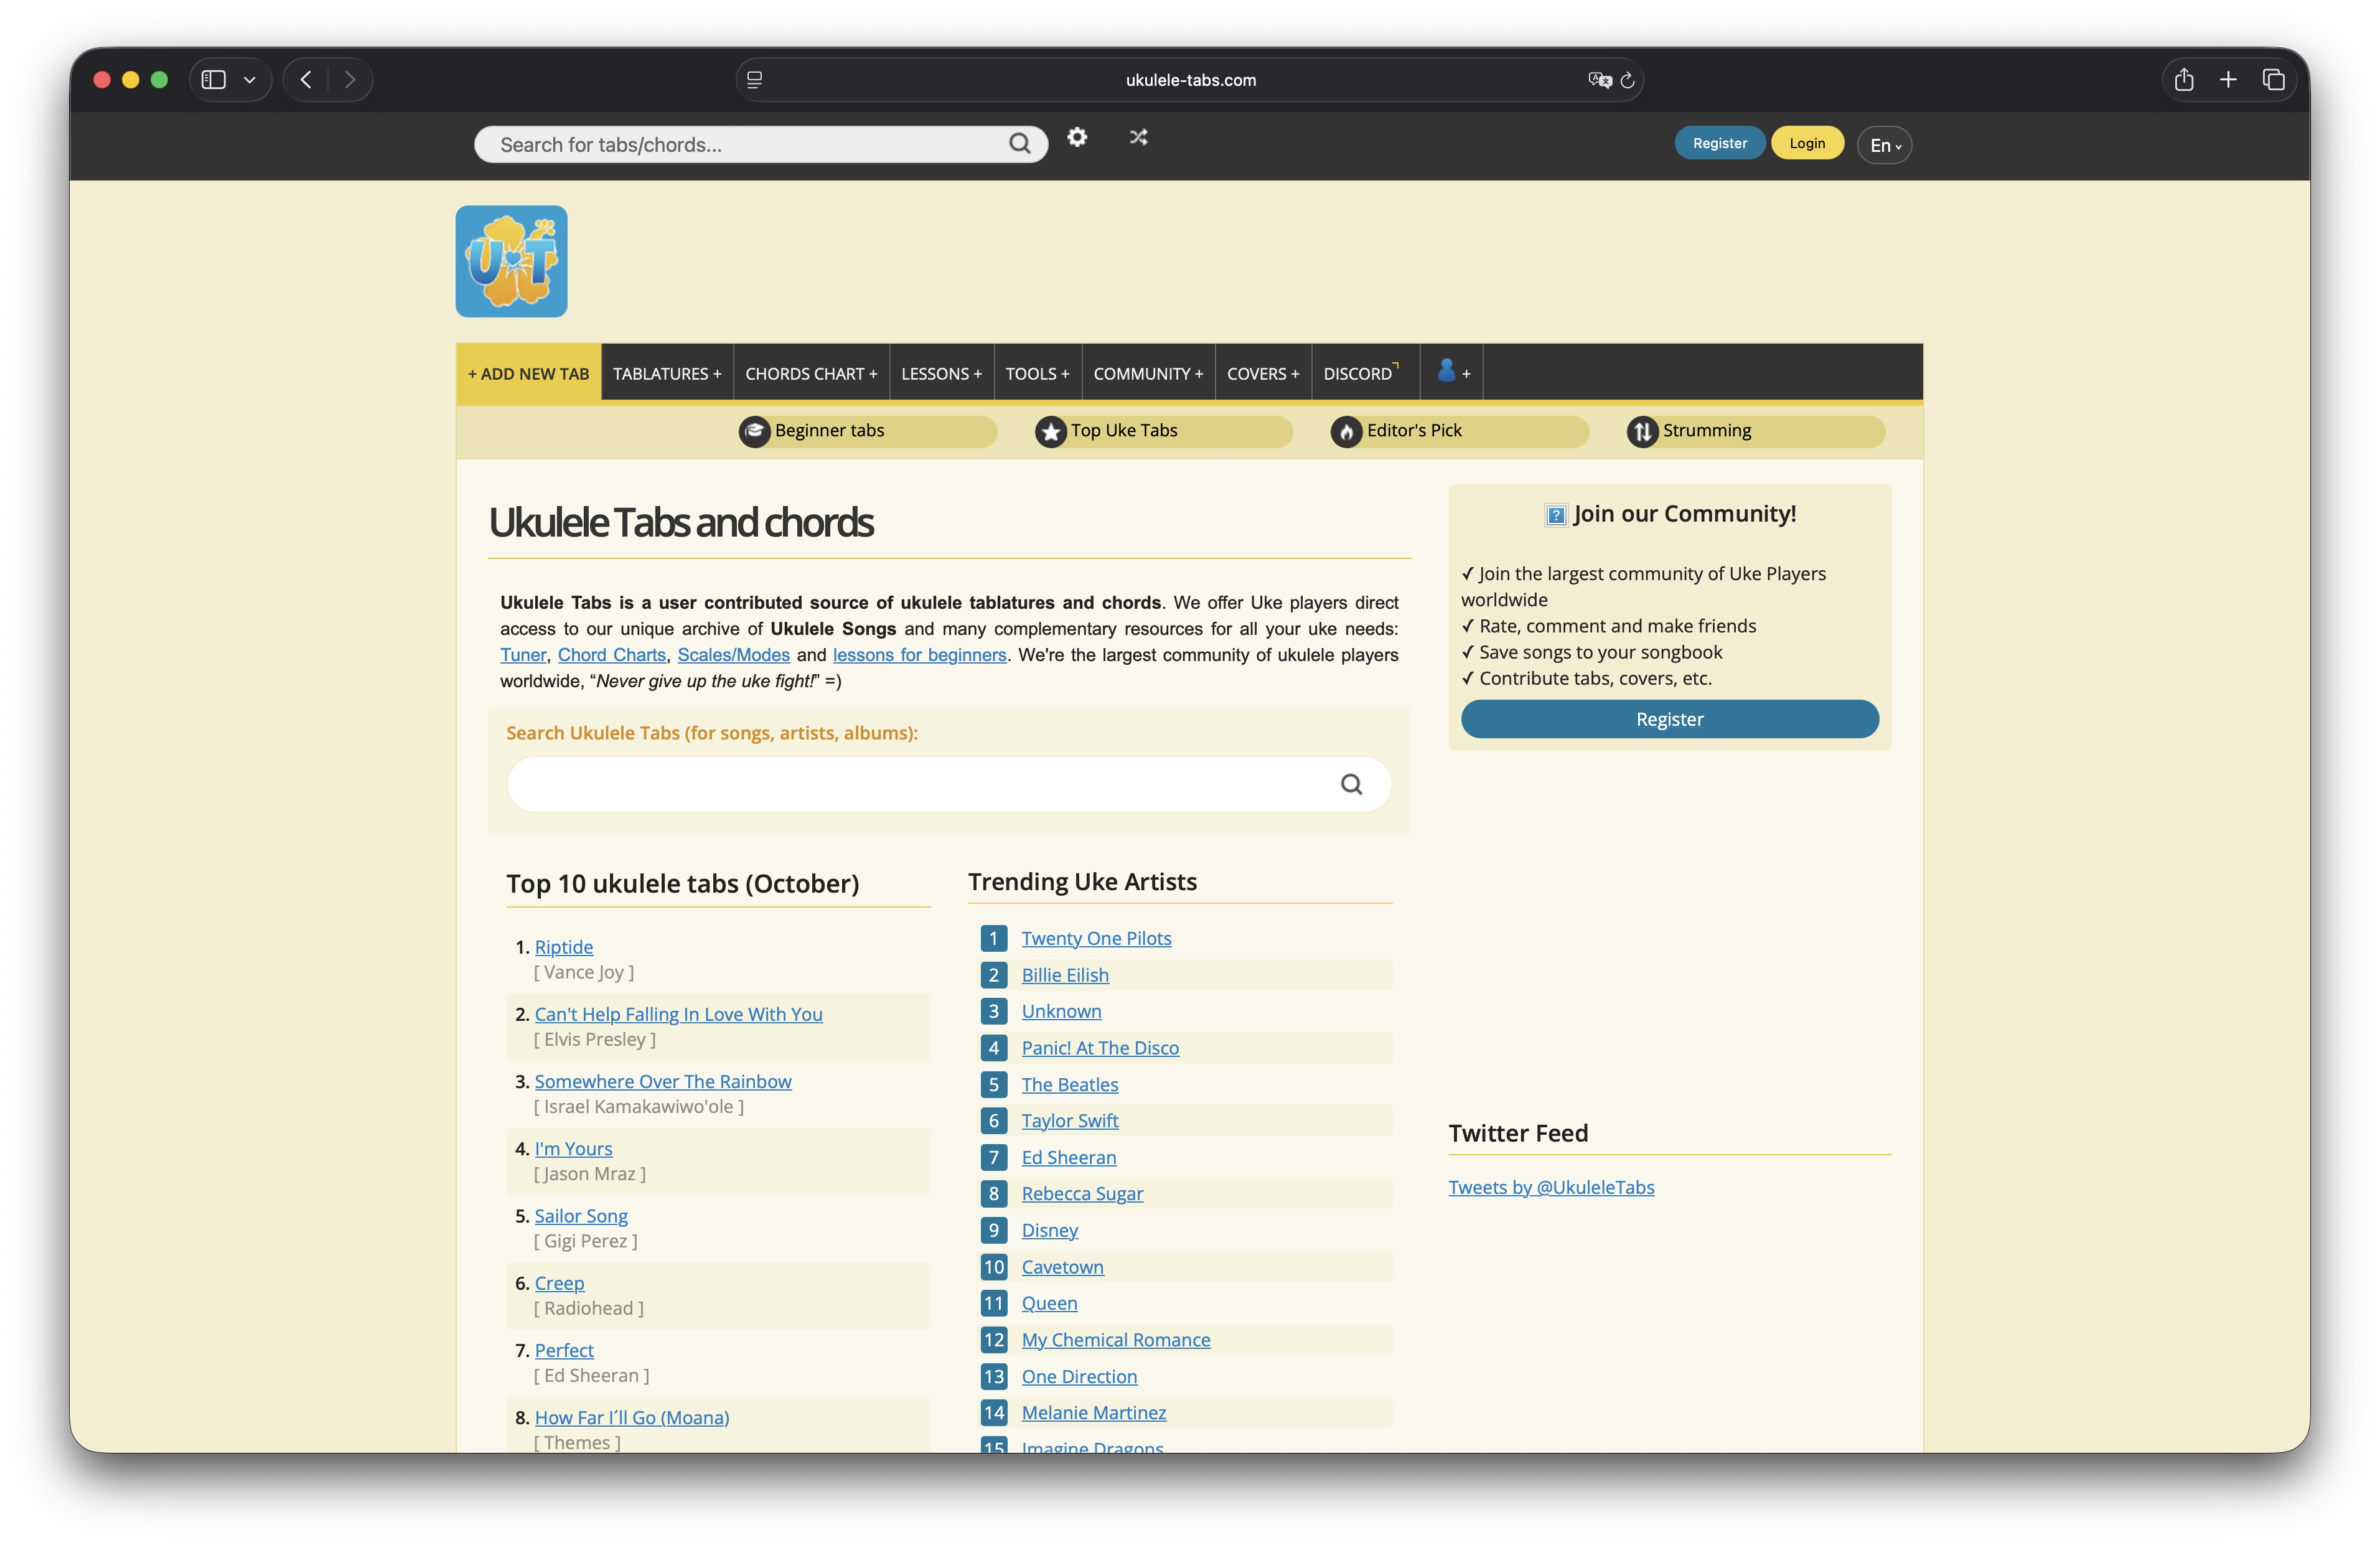
\includegraphics[width=\textwidth]{Ilustraciones/estado/ukuleletabs.jpeg}
        \caption{Página principal de Ukulele Tabs~\cite{ukuleletabs_home}}\label{fig:ukuleletabs_home}
    \end{subfigure}\hfill
    \begin{subfigure}[t]{0.48\textwidth}
        \centering
        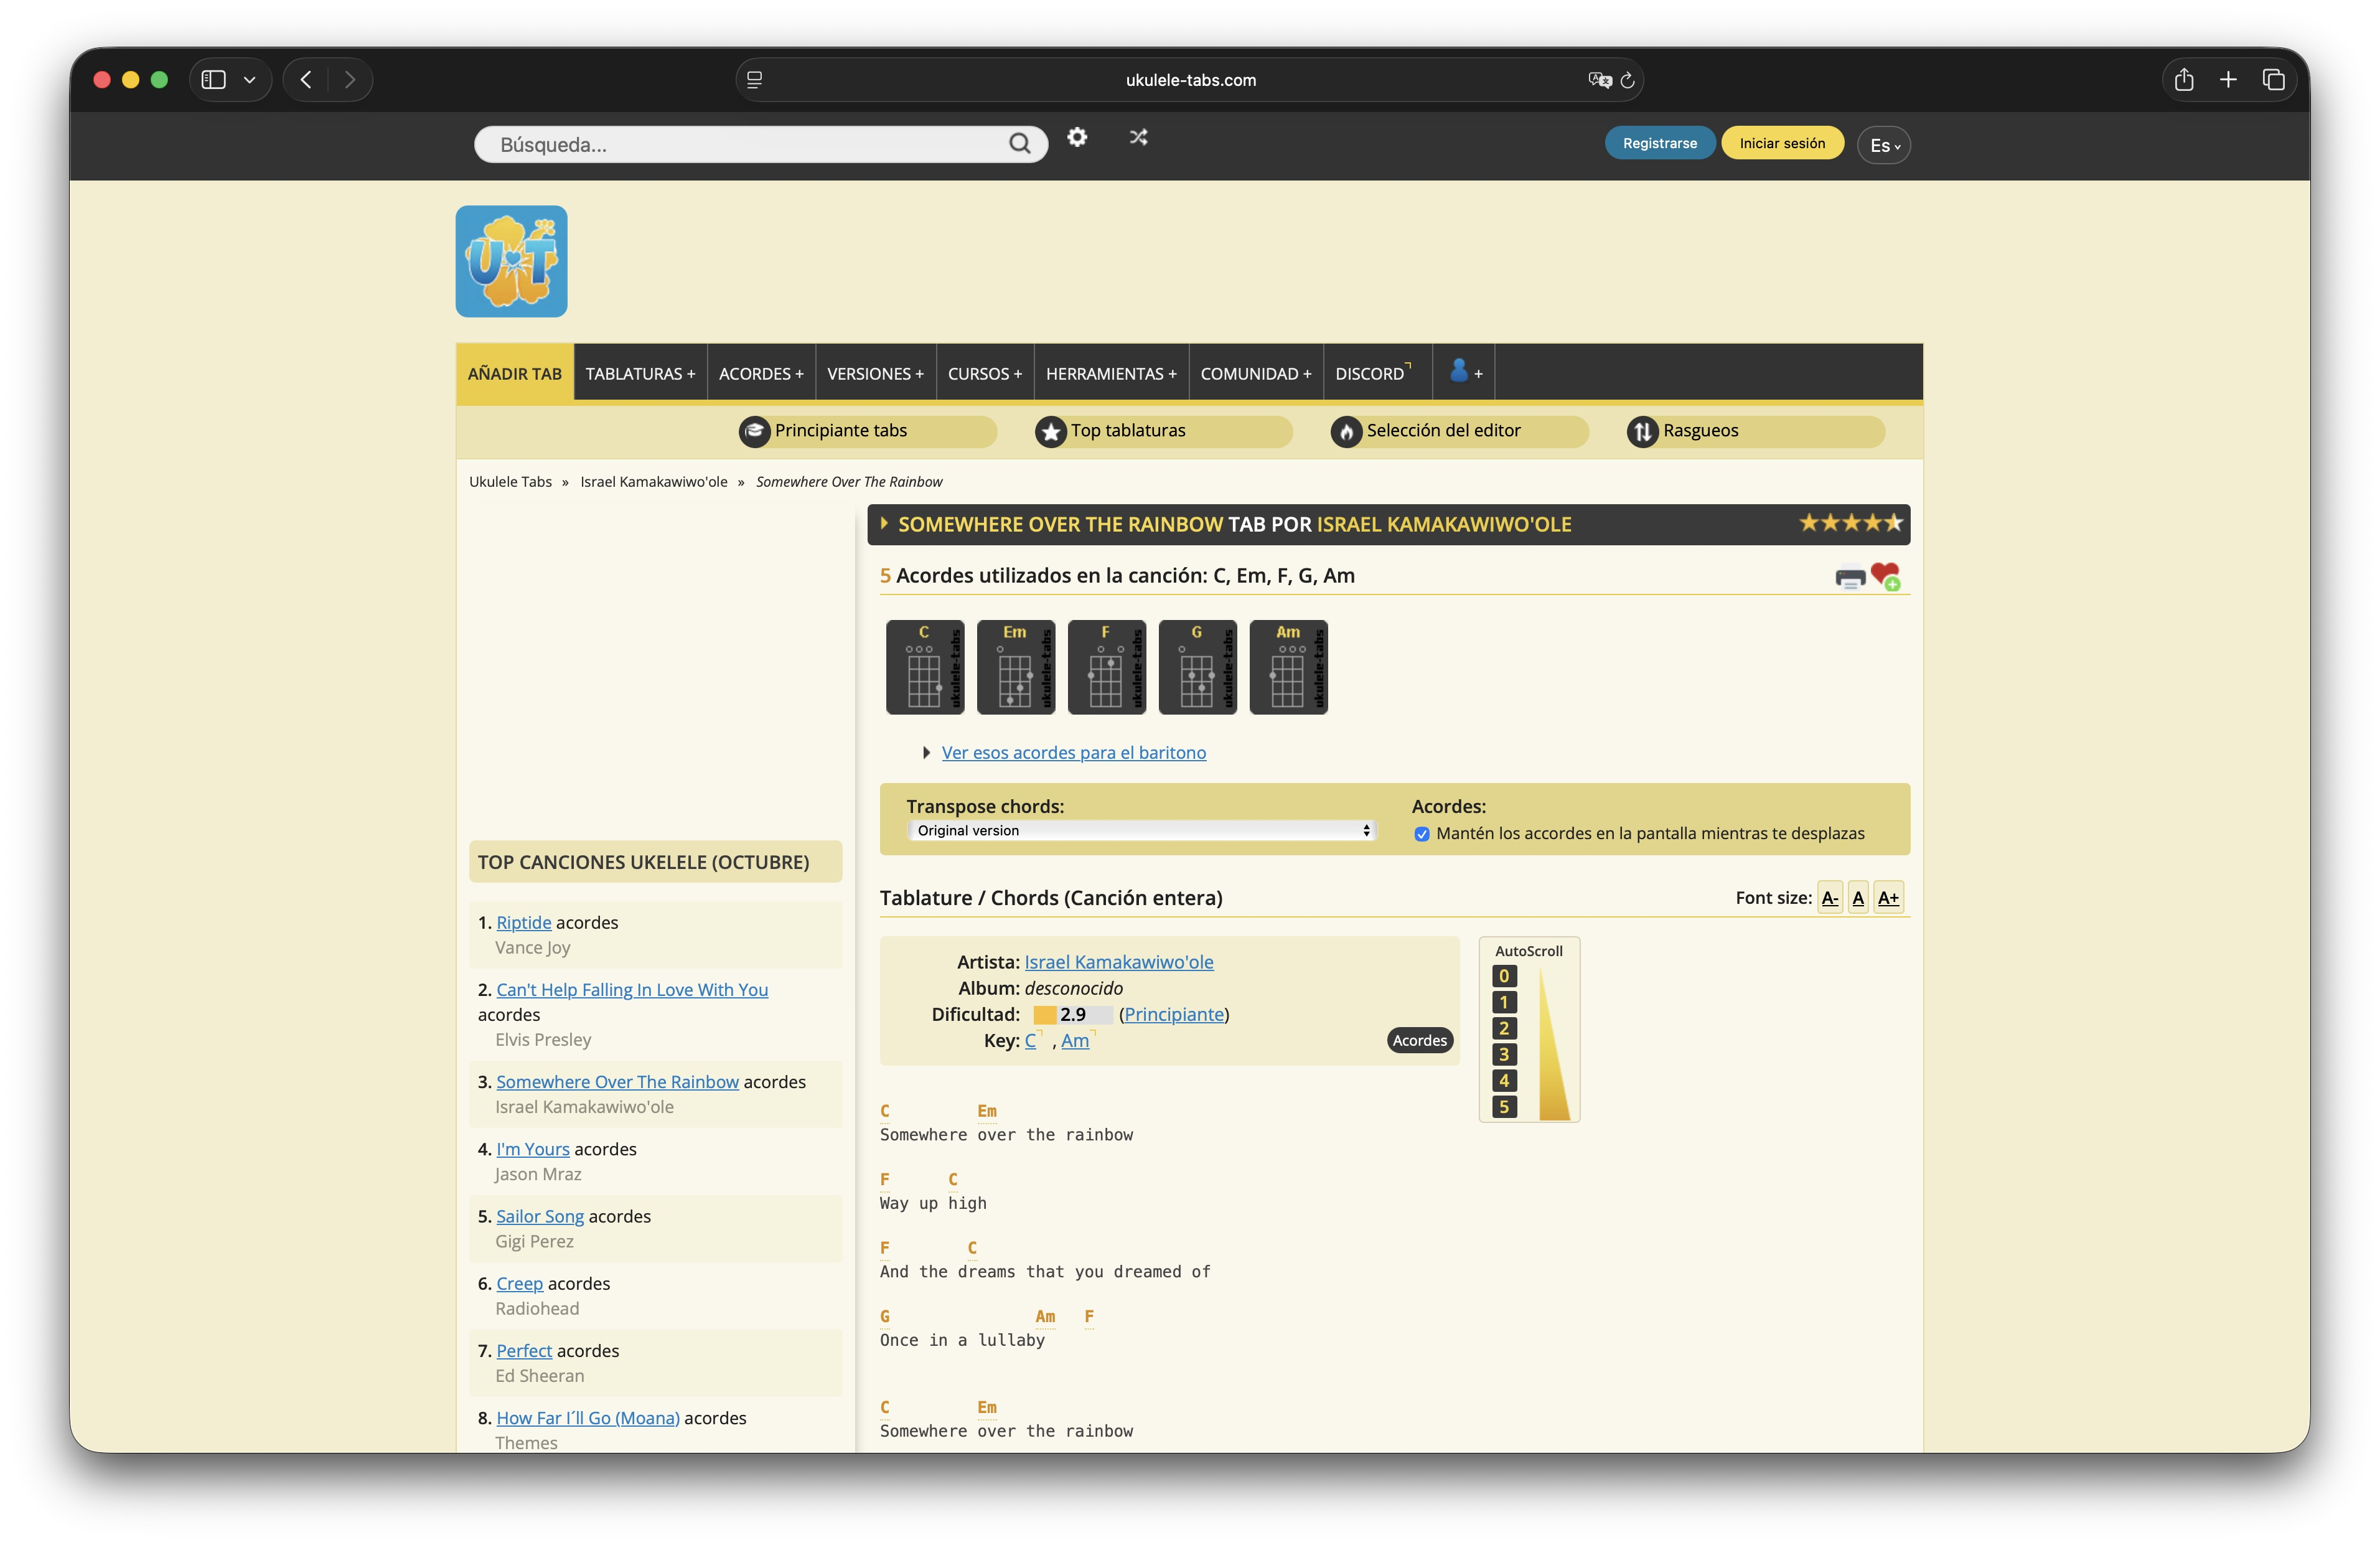
\includegraphics[width=\textwidth]{Ilustraciones/estado/ukuleletabs_somewhereovertherainbow.jpeg}
        \caption{Acordes y letra de \emph{Somewhere over the rainbow} para ukelele en Ukulele Tabs~\cite{ukuleletabs_somewhereovertherainbow}}\label{fig:ukuleletabs_somewhereovertherainbow}
    \end{subfigure}
    \vspace{1em} % Espacio vertical entre filas

    % segunda subfigura
    \begin{subfigure}[t]{0.48\textwidth}
        \centering
        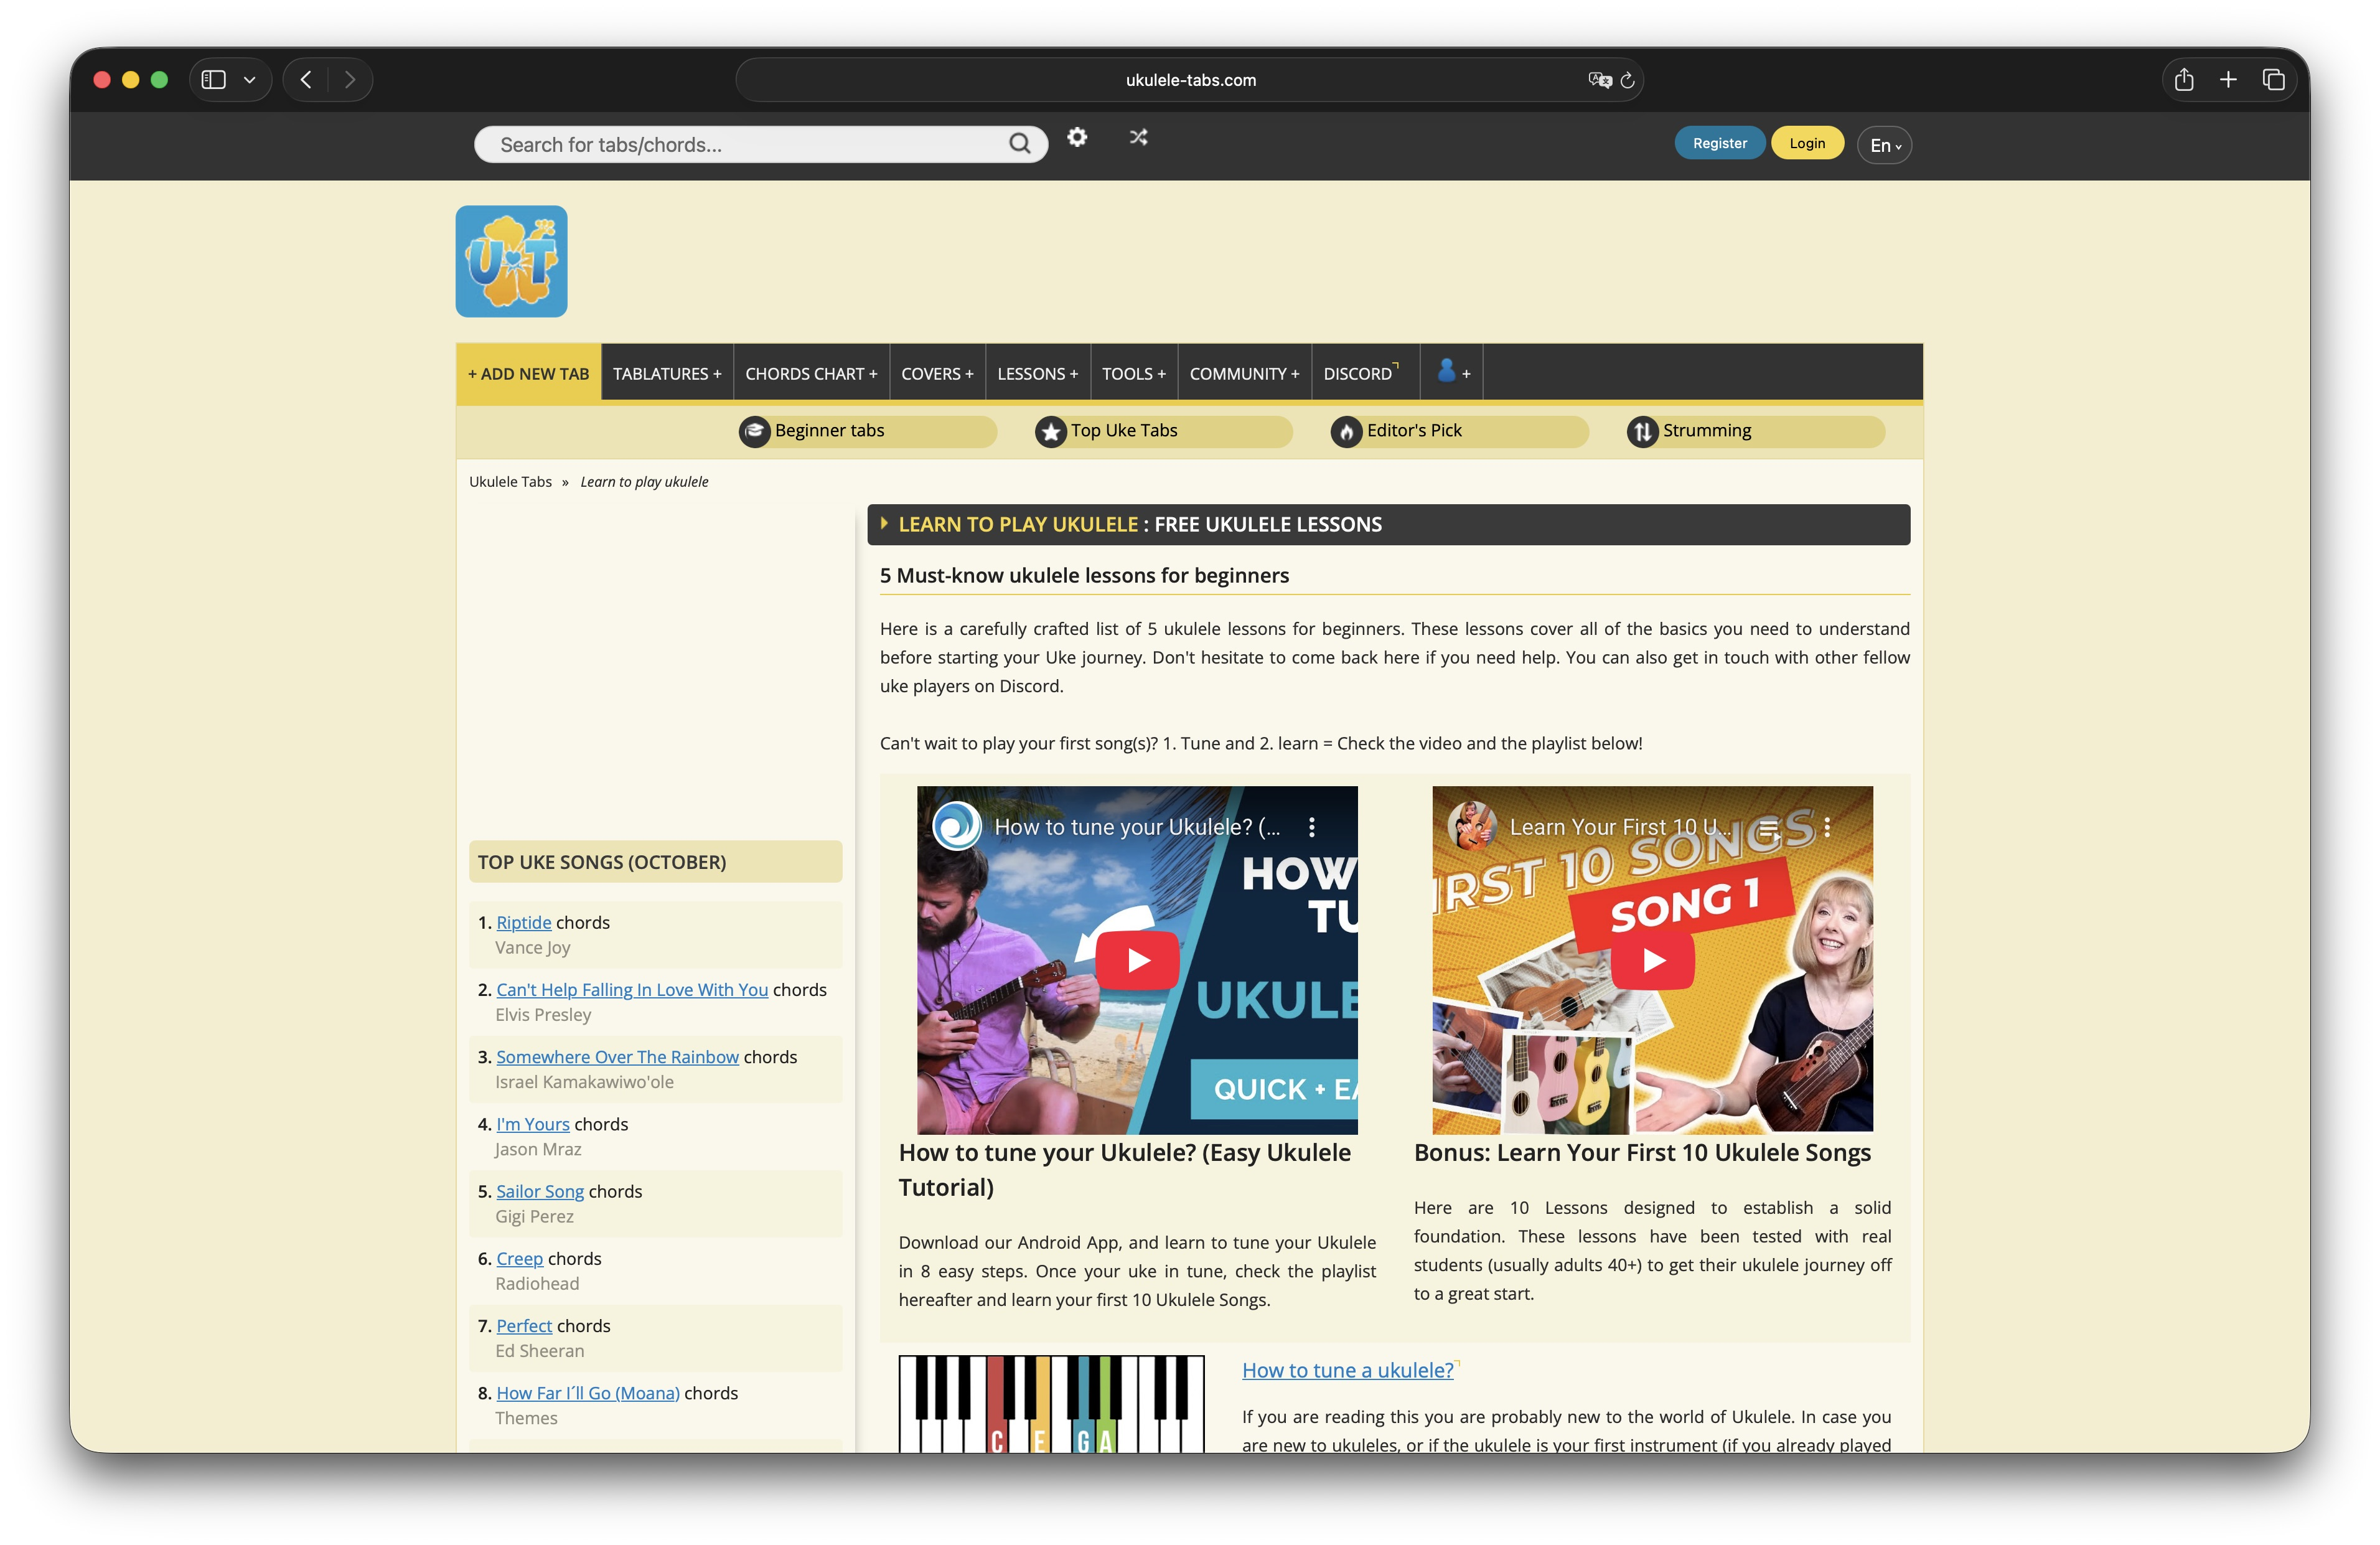
\includegraphics[width=\textwidth]{Ilustraciones/estado/ukuleletabs_lessons.jpeg}
        \caption{Página de cursos de Ukulele Tabs~\cite{ukuleletabs_lecciones}}\label{fig:ukuleletabs_lecciones}
    \end{subfigure}\hfill
    % segunda subfigura
    \begin{subfigure}[t]{0.48\textwidth}
        \centering
        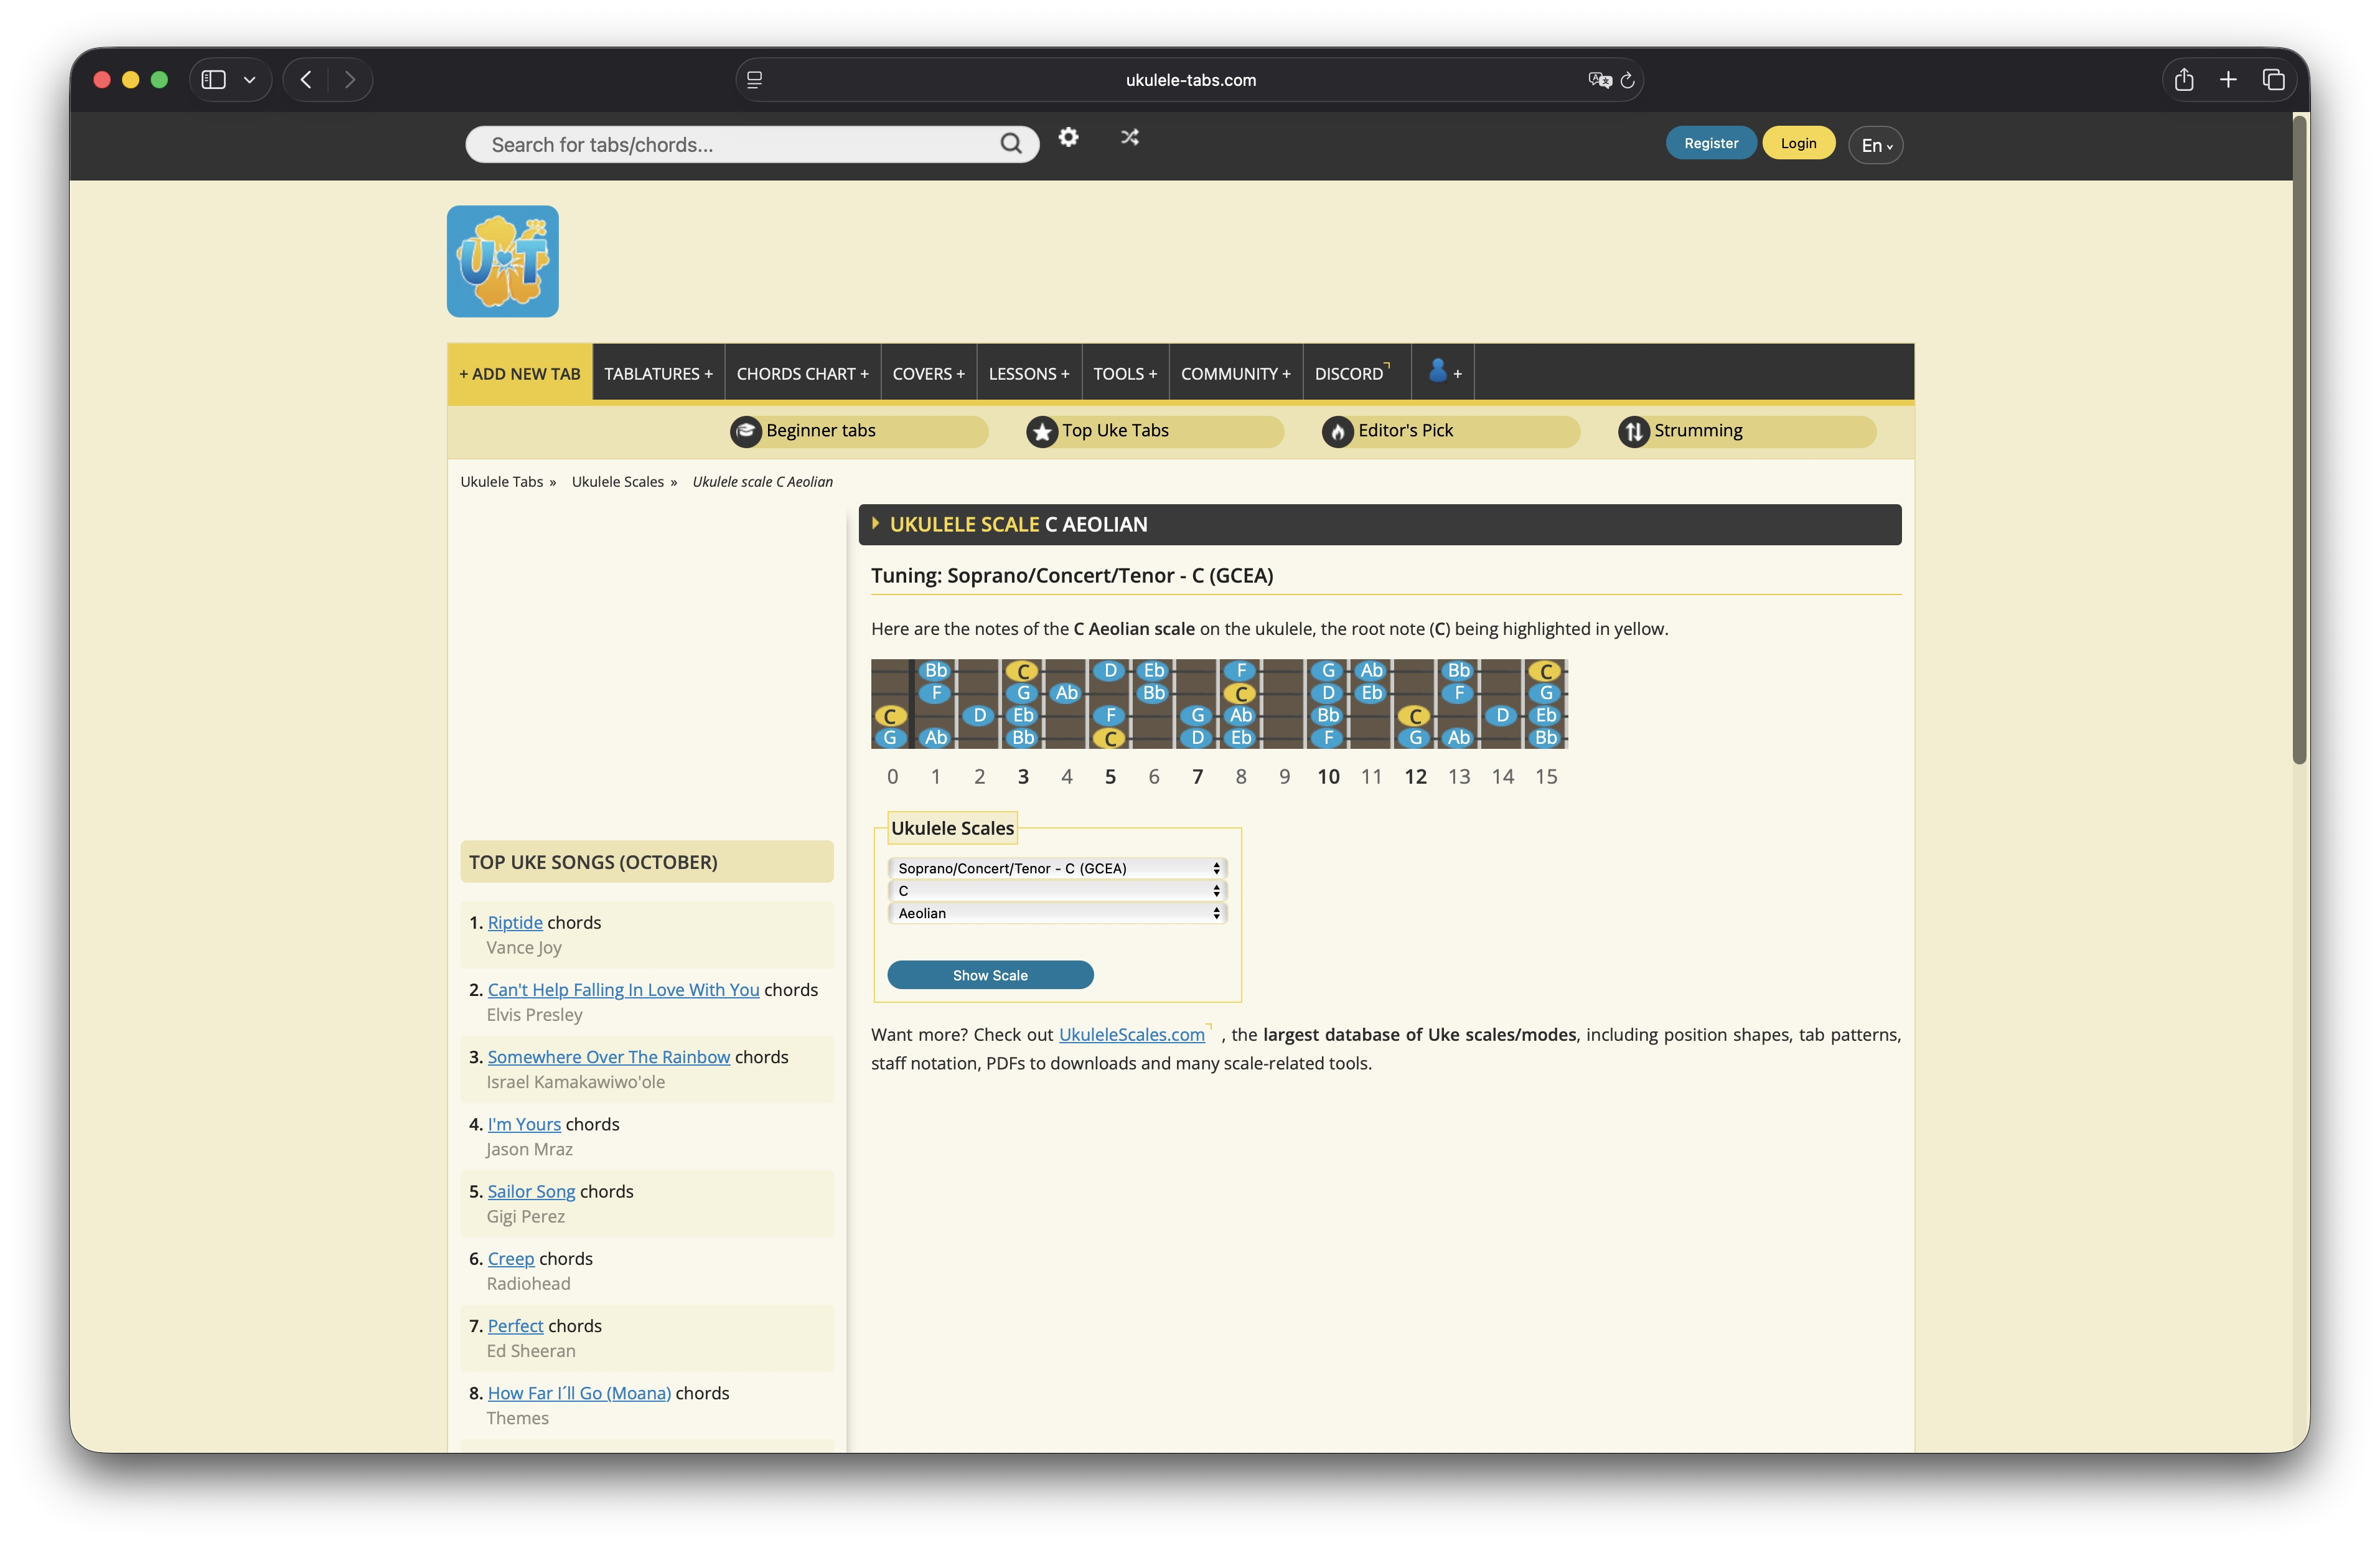
\includegraphics[width=\textwidth]{Ilustraciones/estado/ukuleletabs_escala.jpeg}
        \caption{Página de escalas de Ukulele Tabs~\cite{ukuleletabs_escala}}\label{fig:ukuleletabs_escalas}
    \end{subfigure}

    % caption general
    \caption{Páginas informativas de Ukulele Tabs}\label{fig:ukuleletabs_guias}
\end{figure}

En conclusión, Ukulele Tabs es una aplicación web sencilla y eficaz, con una comunidad activa que contribuye a la verificación del contenido. Aunque no posee un gran número de herramientas y utilidades, sobre todo interactivas, ofrece lo mínimo indispensable para introducirse y practicar con el ukelele. Además, la aplicación se monetiza a través de anuncios publicitarios, lo que permite el acceso gratuito a sus usuarios, poniendo a su disposición la mayoría de sus funcionalidades sin necesidad de registro (veáse Tabla~\ref{tab:ukuleletabs_funcionalidades_usuario}).

\begin{table}[H]
    \centering
    \scriptsize
    \begin{minipage}[t]{0.4\textwidth}
        \centering
        \caption{Utilidades presentes en publicaciones de Ukulele Tabs}\label{tab:ukuleletabs_utilidades_canciones}
        \begin{tabular}{l c}
            \hline
            \textbf{Utilidad} & \textbf{Existe} \\
            \hline
            Transportador & \ding{51} \\
            Lista de acordes & \ding{51} \\
            Autodesplazamiento & \ding{51} \\
            Impresión/Descarga & \ding{51} \\
            Cambio de notación &  \\
            Cambio de instrumento &  \\
            Guardar canción & \ding{51} \\
            Guía de rasgueos & \ding{51} \\
            \hline
        \end{tabular}
    \end{minipage}
    \hfill
    \begin{minipage}[t]{0.56\textwidth}
        \centering
        \caption{Funcionalidades disponibles según el rol del usuario de Ukulele Tabs}\label{tab:ukuleletabs_funcionalidades_usuario}\hfill
        \begin{tabular}{p{0.55\textwidth} c c }
            \hline
            \multirow{2}{*}{\textbf{Funcionalidad}} & \multicolumn{2}{c}{\textbf{Rol Usuario}} \\
             & Visitante & Registrado \\
            \hline
            Biblioteca de canciones & \ding{51} & \ding{51} \\
            Creación y edición de publicaciones &  & \ding{51}  \\
            Utilidades de publicaciones & \ding{51} & \ding{51} \\
            Puntuar publicaciones &  & \ding{51}  \\
            Comentar publicaciones &  & \ding{51}  \\
            Solicitar nuevas canciones &  & \ding{51}  \\
            Cursos y guías & \ding{51} & \ding{51} \\
            Afinador & \ding{51} & \ding{51}  \\
            Calculadora de escalas y notas & \ding{51} & \ding{51}  \\
            Diccionario de acordes & \ding{51} & \ding{51}  \\
            \hline
        \end{tabular}
    \end{minipage}
\end{table}